\documentclass[11pt, a4paper, openany]{book}
\usepackage[utf8]{inputenc}
\usepackage[francais]{babel}
\usepackage[T1]{fontenc}
\usepackage{amsmath}
\usepackage{amsfonts}
\usepackage{amssymb}
\usepackage{lmodern}
%\usepackage{mathpazo}
%\usepackage[scaled=0.95]{helvet}
\usepackage{courier}
\usepackage{amsthm}

\usepackage{graphicx} % ajout image
\usepackage[tt]{titlepic}%Centre le titre

\usepackage{shorttoc} %Permet d'avoir de petites tables des matières


\usepackage{shapepar} %texte en keur
\usepackage{siunitx} %S.I.

\usepackage{graphicx}
\usepackage{caption} %Permet d'ajouter des légendes en images sans les mettre en float + ds la marge
\usepackage{delarray} % Belles matrices

\usepackage{fancyhdr} %Permet de modifier l'entête & footer
\usepackage{bbding} % Note marge
\usepackage{todonotes}
\usepackage{wrapfig}

\pagestyle{headings} % Titre du ch et numéro page dans l'entete
\usepackage{fullpage} %Utilise toute la page
\usepackage{url}
\usepackage{eso-pic} %fond écran page de garde


\newcommand{\cst}{\text{cst}}
\newcommand{\E}{\vec E}
\newcommand{\F}{\vec F}

\newcommand{\questpm}[3]{#1. \textbf{#3} (p.#2)}
\newcommand{\exerc}[2]{\textbf{\Large Exercice #1\normalsize \\#2}}
\newcommand{\dif}{\mathrm{d}}
\newcommand{\comment}[1]{}
\newcommand{\rot}{\text{rot}\,}
\newcommand{\divv}{\text{div}\,}
\newcommand{\phas}[1]{\underline{#1}}
\newcommand{\RE}{\text{Re}}
\DeclareMathOperator{\arccot}{arccot}
\newcommand{\com}[1]{}

%\newcommand{\oiint}{\int\!\!\!\!\!\:\!\!\!\;\!\!\subset\!\!\supset\!\!\!\:\!\!\!\!\!\int}
\newcommand{\oiint}{\int\!\!\!\!\!\!\! \:\!\subset\!\!\supset\!\!\!\!\!\!\!\int}
%%% Background %%%
\newcommand\BackgroundPic{%
\put(0,0){%
\parbox[b][\paperheight]{\paperwidth}{%
\vfill
\centering

\includegraphics[width=\paperwidth,height=\paperheight,%
keepaspectratio]{ulb.jpg}%
\vfill
}}}


\begin{document}
\renewcommand{\proofname}{Démonstration}
\frontmatter
\AddToShipoutPicture*{\BackgroundPic}
\begin{titlepage}
\begin{center}	
	
	\newcommand{\HRule}{\rule{\linewidth}{0.5mm}}   			%Titre en gros
	
\includegraphics[scale=0.11]{logo.jpg}~\\[1cm]				%Logo

	\textsc{\LARGE Université Libre de Bruxelles}\\[1.5cm]
	\textsc{\Large 'Syllabus'}\\[0.5cm]

	\HRule \\[0.4cm]
	{ \huge \bfseries Chimie Physique et Applications Industrielles \\ \ \\ CHIM-H-200 \\[0.4cm] }


	\HRule \\[1.5cm]
		\begin{minipage}{0.4\textwidth}
		\begin{flushleft} \large
		
		\emph{Auteur:}\\
			Nicolas \textsc{Englebert}\\
			\end{flushleft}
			\end{minipage}
			\begin{minipage}{0.4\textwidth}
			\begin{flushright} \large
			\emph{} \\		
			\textsc{}
			\end{flushright}
		\end{minipage}

	\vfill

% Bottom of the page
{\large \today}

\end{center}
\end{titlepage}


\chapter*{Appel à contribution}
\subsection*{Synthèse OpenSource}
\begin{wrapfigure}[5]{l}{4.5cm}
	
\includegraphics[scale=0.5]{git.png}
\end{wrapfigure}
Ce document est grandement inspiré de l’excellent cours donné 
par Marc Haelterman à l’EPB (École Polytechnique de Bruxelles), faculté de l’ULB (Université 
Libre de Bruxelles). Il est écrit par les auteurs susnommés avec l’aide de tous les autres étudiants 
et votre aide est la bienvenue ! En effet, il y a toujours moyen de l’améliorer surtout que si le 
cours change, la synthèse doit être changée en conséquence. On peut retrouver le code source à l’adresse 
suivante
\begin{center}
	\url{https://github.com/nenglebert/Syntheses}
\end{center}\ \\
Pour contribuer à cette synthèse, il vous suffira de créer un compte sur \textit{Github.com}. De
légères modifications (petites coquilles, orthographe, ...) peuvent directement être faites sur le
site ! Vous avez vu une petite faute ? Si oui, la corriger de cette façon ne prendra que quelques 
secondes, une bonne raison de le faire ! \\
\\
Pour de plus longues modifications, il est intéressant de disposer des fichiers : il vous 
faudra pour cela installer \LaTeX, mais aussi \textit{git}. Si cela pose problème, nous sommes 
évidemment ouverts à des contributeurs envoyant leur changement par mail ou n’importe quel autre 
moyen.\\
\\
Le lien donné ci-dessus contient aussi le \texttt{README} contient de plus amples informations, 
vous êtes invités à le lire si vous voulez faire avancer ce projet ! 

\subsection*{Licence Creative Commons}
\begin{wrapfigure}[3]{r}{2.8cm}
	
\includegraphics[scale=0.17]{CC}
\end{wrapfigure}
Le contenu de ce document est sous la licence Creative Commons : \textit{Attribution-NonCommercial-ShareAlike 
4.0 International (CC BY-NC-SA 4.0)}. Celle-ci vous autorise à l'exploiter pleinement, compte-
tenu de trois choses :
\begin{enumerate}
	\item \textit{Attribution} ; si vous utilisez/modifiez ce document vous devez signaler le(s) nom(s)
	      de(s) auteur(s).
	\item \textit{Non Commercial} ; interdiction de tirer un profit commercial de l’œuvre sans 
	      autorisation de l'auteur 
	\item \textit{Share alike} ;  partage de l’œuvre, avec obligation de rediffuser selon la même 
	      licence ou une licence similaire
\end{enumerate}
Si vous voulez en savoir plus sur cette licence :
\begin{center}
	\url{http://creativecommons.org/licenses/by-nc-sa/4.0/}
\end{center}

\begin{flushright}
	\textbf{Merci ! }
\end{flushright}
\tableofcontents

\mainmatter
\part{Chimie Physique}
\chapter{Chimie Physique}
\section*{Chimie Physique ?}
La \textit{chimie physique} est avant tout de la thermodynamique, aussi souvent appelée \textit{thermodynamique chimique}. La définition de cette matière serait :
\begin{center}
\textit{\textsc{Chimie Physique} : cadre conceptuel (et formalisme mathématique) général pour l'étude des transformation de la matière, qu'elles soient chimiques (réactions) ou physiques (changement de phase).} \end{center}

\section{Rappels de thermodynamique}
\begin{wrapfigure}[14]{l}{4.4cm}
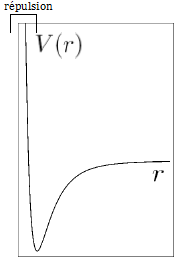
\includegraphics[scale=0.6]{cp/image1.png}
\captionof{figure}{Potentiel d'interaction entre deux molécules en fonction de la distance}
\end{wrapfigure}
La \textit{thermodynamique} est l'étude de variables macroscopiques "collectives" et des relations existant entre elles. S'il fallait calculer le mouvement de chaque particules en utilisant la deuxième loi de Newton, on aurait
\begin{equation}
\ddot{\vec{r_i}} = \frac{1}{m}\sum_{j\neq i} V'(r_{ij}).\vec{e_{ij}}
\end{equation}
La partie $V'(r_{ij}).\vec{e_{ij}}$ n'est qu'une autre notation de la force ($f = -\frac{dV}{dt}$) et $\vec{e_{ij}}$ un vecteur unitaire (la somme représente les forces de toutes les autres particules). Ce calcul n'est pas réalisable pour un grand $(10^6)$ nombre de particules, d'où l'intérêt de la thermodynamique.\\
Le creux de marqué en \textsc{Figure 1.1} montre une distance favorable car il présente le potentiel le plus bas (négatif). C'est favorable car il faudrait appliquer une force pour les "séparer". A partir d'une certaine distance, $V(r)$ devient constant ($V' = 0$) : une particule n'interagit plus avec les autres (plus d'attraction).\\

Pour faire le tri, seules certaines variables (moyennes/macroscopiques) seront utilisées. Parmis celles-ci, deux types :
\begin{enumerate}
\item \textbf{Extensives} $V, n, S, U, ...$ (augmentent avec la taille)
\item \textbf{Intensives} $p, T, s = S/n..$ (indépendantes de la taille)\footnote{On peut obtenir une variable intensive en divisant deux variables extensives}
\end{enumerate}
On utilisera également des \textit{équations d'état}, par exemple la Loi des gaz parfaits:
\begin{equation}
pV = nRT = Nk_BT
\end{equation}
où $R =k_B\,N_A=1,38\times 10^{-23}\,\frac{J}{K}\cdot 6,02\times 10^{23}\,mol^{-1}=8,3\,\frac{J}{mol\, K}$\\
Rappellons que cette première loi avait été obtenue expérimentalement et "vérifiée" une première fois par la théorie cinétique, donnant la "\textit{température cinétique}"\footnote{Comme la loi des gaz parfaits, valable que pour les basses pressions et hautes températures} :
\begin{equation}
pV = Nm\frac{<v^2>}{3}\ \ \ \Rightarrow\ \ \ \frac{3}{2}k_BT = \frac{1}{2}mv^2
\end{equation}
\begin{wrapfigure}[14]{r}{4.4cm}
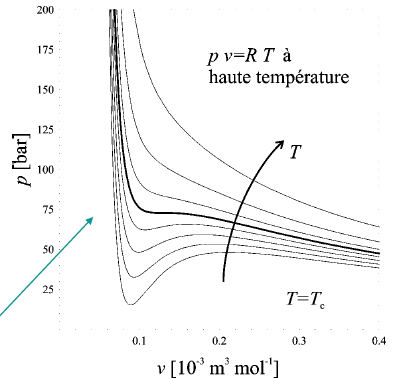
\includegraphics[scale=0.5]{cp/image2.png}
\captionof{figure}{Diagramme de Van der Waals}
\end{wrapfigure}
Il est également possible d'exprimer la loi des gaz parfaits en fonction de la masse volumique $\rho$:
\begin{equation}
\rho = \frac{nM}{V} = \frac{p}{R^*V}\ \ \ \ \ où\ \ R^* = \frac{R}{M}
\end{equation}

Plusieurs généralisations (hors du cas "parfait") sont possibles, comme l'équation du viriel ($p/R^*p : \rho + B(T)\rho^2 + ...$ (développement en série)) ou l'équation de Van Der Waals:
\begin{equation}
\left(p+\frac{a}{v^2}\right)\left(v-b\right) = RT
\end{equation}
La correction sur la pression est due aux interactions entre particules alors que celle apportée au volume (diminution) est causée par la place prise par les particules.\\

On observe sur le Diagramme de Van der Waals ci-contre une sorte de pincement traduisant un phénomène contre-intuitif : pour certaines augmentation du volume, il y a augmentation de la pression.\\

Une autre variable d'état est l'\textbf{énergie thermique} $U$. Celle-ci est répartis entre les différents degrés de libertés (translation, rotation et vibration). La chaleur $Q$ est l'énergie transférée \textbf{au} système et le travail $W$ le travail fourni \textbf{sur} le système.\\

Le \textbf{Premier principe}, traduit que \textit{l'énergie totale est conservée ou l'énergie n'est ni créée ni détruite ou l'énergie d'un système isolé est constante ou ... }. De façon plus générale (forme différentielle):
\begin{equation}
dU = \delta Q + \delta W
\end{equation}
Attention aux convention de signes et au type de système (isolé, ouvert\footnote{Il faudra dans ce cas ajouter $\Delta U_{matière} !$} ou fermé). \\
Attention, $d \neq \delta$, car si $d$ est une différentielle ce n'est pas le cas de $\delta$ car $Q$ et $W$ ne sont pas des fonctions d'état ($\delta$ représente une quantité).\\

N'oublions pas le travail :
\begin{equation}
\delta W = \vec{F}.d\vec{r} = pSdx = -pdV
\end{equation}
Le signe négatif est présent car une diminution du volume augmente la pression : par convention il faut un travail positif, d'où le signe négatif.

Les \textbf{capacités calorifiques} peuvent également jouer. Par définition de celle-ci : $C = \dfrac{\delta Q}{dT}$. Deux cas particuliers sont intéressant (on essaye de changer le $\delta Q$ par une fonction d'état) :
\subsubsection*{A volume constant}
$dV = 0\rightarrow \delta W = 0 \rightarrow \delta Q = dU \Rightarrow$
\begin{equation}
C_V = \left(\frac{\delta Q}{dT}\right)_V = \left(\frac{dU}{dT}\right)_V
\end{equation}

\subsubsection*{A pression constante}
En partant de la définition de l'enthalpie : $H \equiv U + pV$\\
$dH = dU + pdV + \underbrace{Vdp}_0 \rightarrow dH =  dU - \underbrace{dW}_{dU-\delta Q} = \delta Q \Rightarrow$
\begin{equation}
C_p = \left(\frac{\delta Q}{dT}\right)_V = \left(\frac{dH}{dT}\right)_V
\end{equation}
Une rumeur dit qu'il faut connaître les bilans (travail, entropie, ...) des quatre transfmorations élémentaires. Pour rappel :
\begin{enumerate}
\item Isobare (pression constante)
\item Isochore (volume constant)
\item Isotherme (température constante)
\item Adiabatique (pas d'échange de chaleur)
\end{enumerate}

L'étude du \textbf{cycle de Carnot} (cycle réversible) permet de mettre en évidence une relation particulière :
\begin{equation}
\frac{Q_H}{T_H}+\frac{Q_B}{T_B}=0\Rightarrow\oint \frac{\delta Q}{T} = 0
\end{equation}
Voyant ce résultat remarquable, \textit{Clausius} a postulé l'existence d'une fonction d'état\footnote{L'intégrale ne dépend pas du chemin suivi (ne dépend que de l'état dans lequel on se trouve). On dit que $T$ est un facteur intégrant de $\delta Q$.} valant $\frac{\delta Q}{T}$. Il s'agit de l'entropie:
\begin{equation}
S = \int \frac{\delta Q}{T}
\end{equation}
\begin{center}
\textit{\textsc{Second principe :} L'entropie d'un système isolé ne peut qu'augmenter ou rester constante.}
\end{center}
Néanmoins, avec l'expérience on remarque que certaines transformations spontannée (thermalisation, détente irréversible d'un gaz, ...) on toujours un $\Delta S > 0$. Or, pour un système isolé $\delta Q  = 0$ : il doit exister une \textit{source interne} d'entropie:
\begin{equation}
dS = \frac{\delta Q}{T} + d_i S\ \ \ avec\ d_iS \geq 0\ \ \left\{\begin{array}{l}
d_iS > 0\ (processus\ irréversible)\\
d_iS = 0\ (processus\ réversible)
\end{array}\right.
\end{equation}
Dès lors, on peut définir l'\textit{inégalité de Clausius} : 
\begin{equation}
dS \geq \frac{\delta Q}{T}
\end{equation}
\textbf{Un état d'équilibre d'un système isolé est un état d'entropie maximale}.\\


\section{Formule fondamentale de Clausius}
Pour une transformation \textbf{réversible} (système fermé), on connaît les deux premiers principes : $\left\{\begin{array}{l}
dU = \delta Q - pdV\\
dS = \frac{\delta Q}{T}
\end{array}\right.$. En égalant les deux $\delta Q$ pour n'avoir que des fonctions d'état, on obtient la \textit{formule de Clausius} :
\begin{equation}
TdS = dU + pdV
\end{equation}
On peut ré-écrire cette formule en mettant le $dS$ en évidence : $dS = T^{-1}dU + pT^{-1} dV$.\\
Nous savons que l'entropie est une fonction de $U$ et $V$ tel que $S = S(U,V)$. Sa dérivée vaut donc : $dS = \frac{\partial S}{\partial U}dU + \frac{\partial S}{\partial V}dV$. Par identification, on remarque que
\begin{equation}
\frac{1}{T} = \left(\frac{\partial S}{\partial U}\right)_V\ \ \ \ \ \ \ \frac{p}{T} = \left(\frac{\partial S}{\partial V}\right)_U
\end{equation}

\subsection{Application}
Calculons l'entropie d'un gaz parfait. On sait que $\left(\dfrac{\partial S}{\partial V}\right)_U = \dfrac{p}{T} =$\footnote{Loi des gaz parfaits}$ \ \ \ \ \dfrac{nR}{V}$.\\
L'intégration de cette fonction nous donne l'entropie $S$ et une constante.
\begin{equation}
S = f(U) + nR\ln(V)
\end{equation}
Dérivons cette expression par rapport à $U$ pour trouver $f(U)$ comme en \textit{Analyse I} : $\left(\dfrac{\partial S}{\partial U}\right)_V = \dfrac{1}{T} \rightarrow \dfrac{df(U)}{dU} = \dfrac{1}{T}$.
On trouve alors que $df(U) = \frac{dU}{T}$. En multipliant et divisant par $dT$, on voit apparaître l'expression de $C_V$ : $df(U) = \underbrace{C_V}_{dU/dt}\frac{dT}{T}$. On intègre et l'on remplace dans (1.16) :
\begin{equation}
S = a + C_V\ln(T) + nR\ln(V)
\end{equation}
Comme $S$ est extensive, on divise tout par $n$ pour trouver la \textbf{formule de Sackur-Tetrode} (tout en intensive) :
\begin{equation}
\frac{S}{n} = s = s_0 + c_v\ln T + R\ln v\quad\text{où}\left\{\begin{array}{l}
s_0=\frac{a}{n}+R\ln(n)\\
v=V/n\\
c_V=C_V/n
\end{array}\right.
\end{equation}

\subsection{Maximisation de l'entropie}
\subsubsection{Système isolé (mais paroi conductrice et fixe/imperméable) formé de deux sous-systèmes 1  et 2}
\begin{wrapfigure}[7]{l}{3cm}
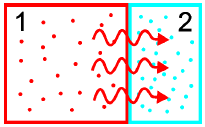
\includegraphics[scale=0.5]{cp/image3.png}
\captionof{figure}{Système isolé fixe}
\end{wrapfigure}
On va simplement appliquer la relation de Clausius pour chaque sous-système :
\begin{equation}
T_idS_i = dU_i + p_idV_i, \ \ \ i= 1,2
\end{equation}
Les parois étant fixe, $dV_i = 0$. Comme l'énergie est conservée $dU = dU_1 +dU_2 = 0$. Ce qui nous donne : 
\begin{equation}
dS = dS_1+dS_2 = \frac{dU_1}{T_1} + \frac{dU_2}{T_2} = dU_1\left(\frac{1}{T_1} - \frac{1}{T_2}\right) \underbrace{\geq 0}_{\underset{\text{principe}}{\text{second}}}
\end{equation}
Lorsque $T_1 = T_2$, on se trouve à l'\textbf{équilibre thermique}.

\subsubsection{Système mobile (parois conductrice et mobile) formé de deux sous-systèmes 1 et 2}
Le principe est le même, si ce n'est qu'ici le volume n'est pas constant. On peut résumer ça : $\left\{\begin{array}{l}
dU = dU_1 + dU_2 = 0\\
dV = dV_1 + dV_2 = 0
\end{array}\right.$. On a donc :
\begin{equation}
dS = dU_1\left(\frac{1}{T_1}+\frac{1}{T_2}\right) + dV_1\left(\frac{p_1}{T_1} - \frac{p_2}{T_2}\right)  \geq 0
\end{equation}
Lorsque $p_1 = p_2$, on se trouve à l'\textbf{équilibre mécanique}.


\subsection{Autres potentiels thermodynamiques (systèmes fermés}
L'énergie libre de Gibbs est définie : 
\begin{equation}
G \equiv H - TS = U + pV - TS\ \ \ \ \ \leq 0 \Leftrightarrow p, T = cste
\end{equation}
L'énergie libre de Helmoltz :
\begin{equation}
F = U - TS\ \ \ \ \ F_{min} \Leftrightarrow T, V = cste\qquad\text{(à l'équilibre)}
\end{equation}

\section{Phases}
\begin{wrapfigure}[7]{r}{2cm}
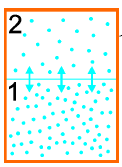
\includegraphics[scale=0.4]{cp/image4.png}
\captionof{figure}{Syst. ouvert}
\end{wrapfigure}
Une phase est une région du système dans laquelle les propriétés sont homogènes (à l'équilibre). Mais attention, dans ce cas on pourrait avoir un système fermé mais constitué de deux sous-systèmes \textbf{ouverts } (échange de matière). Dans ce cas $T_idS_i \neq dU_i + p_idV_i$ et il faut généraliser.

\subsection{Systèmes ouverts (corps purs)}
Ici nous avons donc une variation du nombre de moles $n$, généralisons Gibbs :
\begin{equation}
G(T,p,n) = U + pV - TS
\end{equation}
Rendons $G$ extensive en la divisant par $n$. Cela donne ce que l'on appelle le \textbf{potentiel chimique $\mu$}:
\begin{equation}
\frac{G}{n} = g(T, p) = \mu(T,p)
\end{equation}
Dérivons encore une fois comme en \textit{Analyse I} :\\
 $dG = \left(\dfrac{\partial G}{\partial T}\right)_{p,n} dT + \left(\dfrac{\partial G}{\partial p}\right)_{T,n} dp +  \left(\dfrac{\partial G}{\partial n}\right)_{T,p}dn$. Pour la dérivée en $n$, on utilise : $G = n.\mu$ et pour le reste on dérivée (1.22). On en tire :
\begin{equation}
dG = -SdT + Vdp + \mu dn
\end{equation}
Avec le potentiel, Gibbs est maintenant à deux variable = $G(n,\mu)$. Sa dérivée vaut donc $dG = nd\mu + \mu dn$. Isolons $d\mu = \dfrac{dG - \mu dn}{n}$. A l'aide de (1.25) on peut conclure :
\begin{equation}
d\mu =\left(\frac{\partial\mu}{\partial p}\right)_Tdp+\left(\frac{\partial\mu}{\partial T}\right)_pdT= -sdT + vdp\Rightarrow\left\{\begin{array}{l}
\left(\dfrac{\partial \mu}{\partial p}\right)_T = v\\
\left(\dfrac{\partial \mu}{\partial T}\right)_p = -s
\end{array}\right.
\end{equation}
\subsubsection{Autres formules fondamentales}
Nous connaissons maintenant deux expression de $dG$ :
\begin{eqnarray}
dG &=& d(\underbrace{U + pV}_H - TS) = dU + pdV + Vdp - TdS - SdT\\
dG &=& -Sdt + Vdp + \mu dn
\end{eqnarray}
En égalant les $dG$ on trouve la \textbf{relation de Gibbs} pour un système \textbf{ouvert} formé d'un corps pur.
\begin{equation}
TdS = dU + pdV - \mu dn
\end{equation}
En faisant mumuse avec les variables, on peut dire que $G = n\mu = U + pV - TS \rightarrow \mu = u + pv - Ts$ qui n 'est formé que de variables intensives.\\
L'enthalpie molaire : $h = \frac{H}{n} = \frac{U + pV}{n} \rightarrow \mu = h - Ts$.

\subsection{Équilibre chimique}
On procède comme pour l'équilibre thermique et mécanique (parois conductrice de chaleur, mobile et perméable ; système isolé composé de 2 sous-systèmes ouverts) :
\begin{equation}
T_idS_i = dU_i + p_idV_i - \mu_idn_i\quad\text{où}\quad\left\{\begin{array}{l}
dU = dU_1 + dU_2 = 0\quad\text{(système isolé)}\\
dV = dV_1 + dV_2 = 0\quad\text{(variation de volume entre les sous-systèmes)}\\
dn = dn_1 + dn_2 = 0\quad\text{(pas d'échange de matière)}
\end{array}\right.
\end{equation}
Ce qui nous donne : 
\begin{equation}
dS = dU_1\left(\frac{1}{T_1}-\frac{1}{T_2}\right) + dV_1 \left(\frac{p_1}{T_1}-\frac{p_2}{T_2}\right) + dn_1\left(\frac{\mu_2}{T_2}-\frac{\mu_1}{T_1}\right) \geq 0
\end{equation}
Lorsque $\mu_1 = \mu_2$, on se trouve à l'\textbf{équilibre chimique}.\\
L'équilibre thermodynamique est donc composé de trois équilibres (vers le potentiel chimique le + bas).

\subsection{Équilibre entre phases pures}
A l'équilibre, le potentiel d'une phase vaut celle de l'autre : $\mu_1(T, p) = \mu_2(T,p) \rightarrow -s_1dT + v_1dp = -s_2dT + v_2dp \Rightarrow$
\begin{equation}
\frac{dp}{dT} = \frac{s_1 - s_2}{v_1 - v_2}
\end{equation}
Comme $\mu_1 = h_1 - Ts_1 = \mu_2 = h_2 - Ts_2$ on trouve la \textbf{relation de Clapeyron :}
\begin{equation}
\frac{dp}{dT} = \frac{1}{T}.\frac{h_1 - h_2}{v_1 - v_2} = \frac{\Delta h}{T\Delta v}
\end{equation}
où $\Delta h:=$ chaleur latente
\subsubsection{Équilibre liquide-vapeur}
Prenons comme hypothèse que la vapeur est un gaz parfait et que $v_{vap} >> v_{liq}$ :
\begin{equation}
\frac{dp}{dT} = \frac{1}{T}.\frac{h_{vap} - h_{liq}}{v_{vap} - v_{liq}} \simeq \frac{h_{vap} - h_{liq}}{Tv_{vap}}
\end{equation}
Comme $p.v_{vap} = RT$ (gaz parfait), on trouve la loi de \textbf{Clausius-Clapeyron}:
\begin{equation}
\frac{dp}{dT} = \frac{\mathcal{L}}{RT^2}p
\end{equation}
Ou encore ($\mathcal{L} = h_{vap} - h_{liq}$, la chaleur latente de vaporisation (considérée cste sur la gamme de température)) :
\begin{equation}
\ln\left(\frac{p}{p_0}\right) = -\frac{\mathcal{L}}{R}\left(\frac{1}{T}-\frac{1}{T_0}\right)
\end{equation}

\subsubsection{Ébullition ou évaporation ?}
\begin{wrapfigure}[8]{r}{2cm}
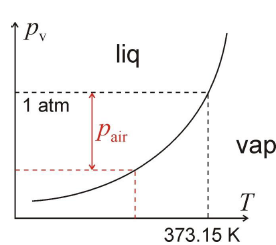
\includegraphics[scale=0.4]{cp/image5.png}
\captionof{figure}{Équilibre liquide-vapeur}
\end{wrapfigure}
On sait qu'à $1\ atm$ l'eau bout à 100 degrés. Mais l'eau n'a pas besoin d'être si chaude pour s'évaporer. Ou est la différence ?\\
L'ébullition est la croissance de bulles de vapeur pur ayant une pression d'$1\ atm$. Par contre, l'évaporation dans l'air (= mélange) : la \textit{vaporisation} se fait à $T_{vap} < 373.15\  K$ car $p_v = 1\ atm - P_{air}$.\\

On peut ainsi dire que :\\
La présence d'un gaz inerte (tel que l'air) ne modifie pas les conditions d'équilibre \emph{pour autant que :}
\begin{itemize}
\item la pression partielle de l'air ne soit pas trop élevée
\item la pression à considérer est la pression partielle $p_v$
\end{itemize}
Ainsi, si on venait à souffler sur un liquide celui-ci s'évaporerait plus rapidement (car augmente la pression et diminue ainsi la température de changement de phase)

\subsubsection*{Règles des phases de Gibbs}
Rapide rappel du cours de \textit{Chimie générale}. Celle-ci s'énonce\footnote{$w$ est (plus formellement) le nombre de variables intensives indépendantes (= nécessaire pour connaitre toutes les autres)} :
\begin{equation}
w = 2 + c - \phi - r\ \ \ où\ \ \left\{\begin{array}{l}
w = \text{variance = nbre de degrés de liberté}\\
c = \text{nombre de constituants}\\
\phi = \text{nombre de phases}\\
r = \text{nombre d'équilibres chimiques}
\end{array}\right.
\end{equation}
Pour un corps pur, $c=1, r=0$ : $w = 3 - \phi$. Selon la valeur de $\phi (1,2,3)$ le sytème sera dit \textit{bivariant, monovariant} (droite) ou \textit{invariant} (point triple).\\
Trois phases en équilibre n'ont donc pas de degré de liberté et si deux phases sont en équilibre, on a toujours une contrainte additionnelle.
\newpage
\subsubsection{Diagrammes des phases}
\textsc{Dioxyde de carbone}\\
\begin{wrapfigure}[12]{l}{8cm}
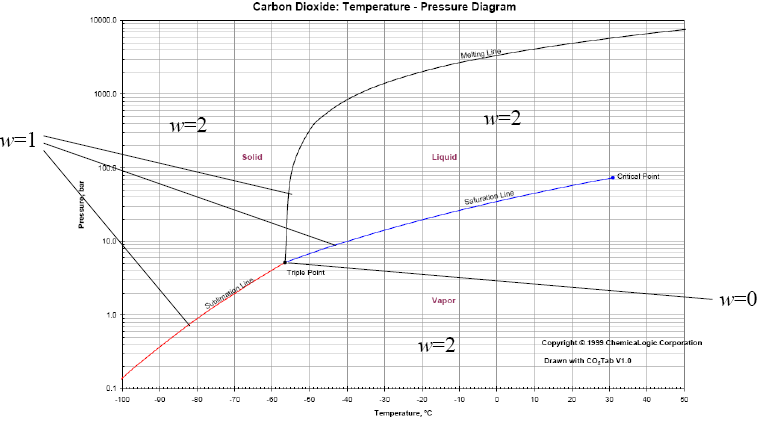
\includegraphics[scale=0.37]{cp/image6.png}
\captionof{figure}{Diagramme des phases $CO_2$}
\end{wrapfigure}
Une différence importante par rapport à l'eau est que la pente d'équilibre liquide \textit{solide-liquide} est positive. A température ambiante il n'y a pas de phase liquide : on observe directement la sublimation.\\

\textsc{Eau}\\
Par manque de place je n'inclus pas le diagramme. On remarque cependant qu'à \textbf{très} haute pression la pente \textit{solide-liquide} devient positive : la glace se contracte en se solidifiant. C'est du au fait qu'à haute pression la glace tente de diminuer son volume et un réseau de type cristal (minimisant le volume) se forme.

\newpage
\textsc{Carbone}\\
\begin{wrapfigure}[12]{r}{5cm}
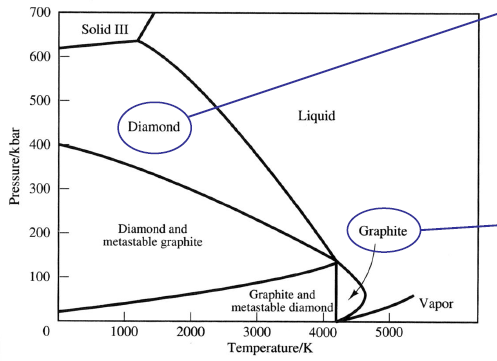
\includegraphics[scale=0.37]{cp/image7.png}
\captionof{figure}{Diagramme des phases carbone}
\end{wrapfigure}
Le diamant "stable" n'existe qu'à haute pression et température. A température et pression ambiante on peut avoir formation de graphique et de diamant \textit{métastable}.\\
Métastable désigne une forme de phase qui a un potentiel possible mais qui est supérieur au potentiel d'une autre phase également présente : ce n'est pas le plus "spontané". \\

Pourquoi alors avons-nous du diamant à $T$ et $p$ ambiant alors que $\mu_{diamant} > \mu_{graphite}$ ?  Car la transformation est extrêmement lente et qu'il y a une barrière d'énergie : il faut casser les liaisons ce qui est énergivore.

\subsection{Equation d'état de Van der Waals}
\begin{wrapfigure}[12]{r}{2cm}
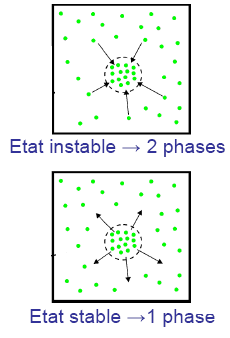
\includegraphics[scale=0.37]{cp/image8.png}
\captionof{figure}{Stable/instable}
\end{wrapfigure}
Un gaz réel possède une transition liquide vapeur dont la pression est donnée par une belle équation déjà vue un peu plus haut :
\begin{equation}
p = \frac{RT}{v-b}-\frac{a}{v^2}
\end{equation}

En étudiant la variation de la pression par rapport au volume à température constante, deux cas sont possible\footnote{} :
\begin{equation}
\left(\frac{\partial p}{\partial v}\right)_T\ est\ \ \left\{\begin{array}{l}
< 0 : stable\rightarrow 1\ phase\\
> 0 : instable\rightarrow 2\ phases
\end{array}\right.
\end{equation}
\begin{wrapfigure}[15]{l}{6cm}
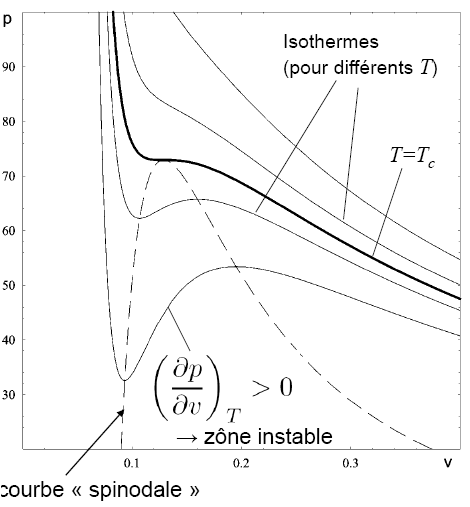
\includegraphics[scale=0.35]{cp/image9.png}
\captionof{figure}{Courbe spinodale}
\end{wrapfigure}
Si la dérivée est positive, c'est que l'on se trouve dans le cas spécial ou $P$ augmente avec $V$ (contre-intuitif) et que deux phases sont présentes. Si ce n'est pas le cas, on observe bien une diminution de la pression avec l'augmentation du volume (effet "normal", PV = cste pour un gaz parfait).
\\
Égalons cette dérivée à zéro. On obtient dès lors : 
\begin{equation}
RT = 2av^{-3}(v-b)^2
\end{equation}

En isolant $RT$ dans l'expression de Van der Waals ci-dessus et en le remplaçant ici, on obtient :
\begin{equation}
p_{sp} = av^{-3}(v-2b)
\end{equation}
qui est la \textbf{courbe "spinodale"}, c'est à dire la courbe qui détermine les états instables\footnote{A l'intérieur de la courbe spinodale : A l'extérieur : stable.} qui mène spontanément à la formation de deux phases : liq. et vap. Sous cette courbe, on voit que $P$ augmente avec $V$ (cf. plus haut).




\begin{wrapfigure}[15]{l}{9.5cm}
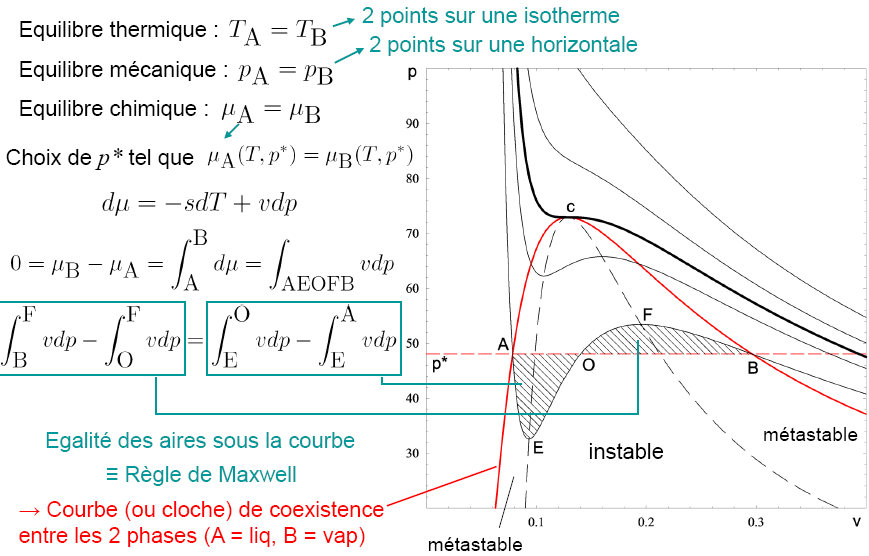
\includegraphics[scale=0.4]{cp/image10.png}
\captionof{figure}{Règle de Maxwell}
\end{wrapfigure}
Une isotherme est défini par une température constante : deux points sur une isotherme ont donc la même température. Pour une même pression ($y = cste$) on se trouve à l'équilibre mécanique. L'équilibre chimique correspond à $\mu_A = \mu_B$.\\

On cherche un $p^*$ tel que $\mu_A(T,p^*) = \mu_B(T,p^*)$. Sachant que $d\mu = -sdT + vdp$ et que le potentiel étant une fonction d'état, on peut choisir le chemin suivi : prenions le chemin $AEOFB$ pour rester sur la couche à température constante. Comme $\Delta \mu = 0$ on peut développer l'intégrale sur le chemin et réorganiser les membres pour trouver la \textbf{règle de Maxwell}.
\begin{equation}
\int_B^F vdp - \int_O^F = \int_E^O vdp - \int_E^A vdp
\end{equation}
Celle-ci donne la courbe (ou cloche) de coexistence entre les deux phases ($A$ = liq, $B$ = vap)

\subsubsection{Stabilité et métastabilité}
Un état est \textit{instable} s'il évolue vers un autre état à la suite d'une perturbation aussi petite soit-elle.\\
Un état est \textit{métastable} s'il est stable pour de petites perturbation\footnote{Stable localement}, mais évolue vers un autre état à la suite d'une perturbation assez grande (présence d'une barrière surchauffée).

\subsection{Tension superficielle}
La tension superficielle est la manifestation des forces moléculaires. Les molécules placée dans le liquide  ont un état plus favorables que celles à la surface ($1/2$ fois moins d'interactions). Comme la surface est moins favorable, l'augmenter nécessite de fournir un travail :
\begin{wrapfigure}[7]{l}{3.5cm}
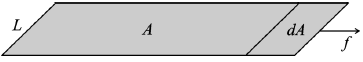
\includegraphics[scale=0.4]{cp/image12.png}
\captionof{figure}{Agrandissement $dA$}
\end{wrapfigure}
\begin{equation}
dU_{surf} = fdx = \frac{f}{L}dA = \underbrace{\gamma dA}_{\text{Energie de surface}}
\end{equation}
où $\gamma$ est la \textit{tension superficielle}. La "liaison" entre la surface $A$ et l'agrandissement $dA$ est séparé par l'\textit{interface}.\\
Pour un système formé de deux phases 1 et 2 en contact (\textbf{Hypoth.} : Température uniforme et transfo. réversible), nous savons grâce à la relation de Clausius\footnote{$TdS = dU + pdV$} : 
\begin{eqnarray}
dU &=& dU_1 + dU_2 + dU_{surf}\\
 &=& TdS - p_1dV_1 - p_2dV_2 + \gamma dA
\end{eqnarray}
Notons que la forme sphérique se manifeste dans le but d'augmenter les forces de cohésions, en minimisant la surface.

\subsubsection{Loi de Laplace}
Prenons l'énergie libre de Helmholtz ($dF = dU - TdS - SdT$) et remplaçons-y l'expression de $dU$ obtenue ci-dessus. Les $TdS$ se simplifient pour donner :
\begin{equation}
dF = -SdT - p_1dV_1 - p_2dV_2 + \gamma dA
\end{equation}
Si $T, V_1$ et $V_2$ sont constant, on peut en tirer :
\begin{equation}
\gamma = \left(\frac{\partial F}{\partial A}\right)_{T, V_1, V_2} > 0
\end{equation}
\begin{wrapfigure}[9]{r}{4cm}
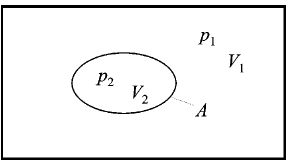
\includegraphics[scale=0.4]{cp/image13.png}
\captionof{figure}{Phase 1 et 2}
\end{wrapfigure}
Imaginons un système composé de deux phases, ou la phase 2 se trouve inclue dans la phase 1. Si $V$ et $T$ sont constant, on sait que $dV_1 + dV_2 = 0$. Maximisons $dF$ en l'égalant à zéro :
\begin{equation}
dF = (p_1 - p_2)dV_2 + \gamma dA
\end{equation}
En supposant que la phase 2 reste sphérique : $V_2 = \frac{4}{3}\pi R^3, A = 4\pi R^2$ ce qui implique que $dV_2 = 4\pi R^2 dR$ et $dA = 8\pi R dR$. En remplace, on simplifie les $4\pi$ et $dR$ pour finalement avoir la \textbf{moi de Laplace pour une sphère} (bulle, goutte, ...) :
\begin{equation}
p_2 - p_1 = 2\frac{\gamma}{R}
\end{equation}
On avait vu précédemment pourtant que l'équilibre se produisait lorsque $p_1 = p_2$, est-ce toujours valable ? Oui, car avant nous avions des surfaces planes ce qui n'est plus le cas ici ! (Si $R \rightarrow \infty$ on retrouve bien l'équilibre mécanique). 
La loi de Laplace est donc une généralisation de la condition d'équilibre mécanique. On peut montrer géométriquement que son expression est semblable à :
\begin{equation}
p_2 - p_1 = \gamma\left(\frac{1}{R_1} + \frac{1}{R_2}\right)
\end{equation}

\subsubsection{Mouillage}
Il s'agit de la tendance d'un liquide à s'étaler ce qui dépend de l'affinité moléculaire du solide avec les molécules du liquide. 
\begin{center}
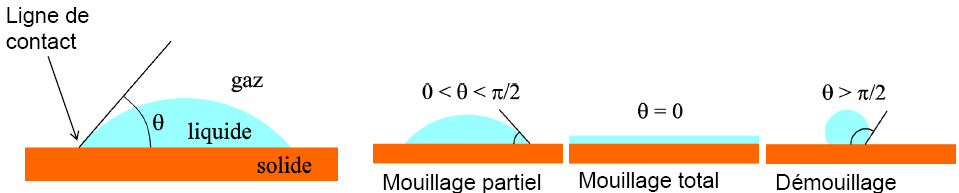
\includegraphics[scale=0.5]{cp/image14.png}
\captionof{figure}{Ligne de contact - Type de mouillage}
\end{center}
\begin{wrapfigure}[9]{R}{4cm}
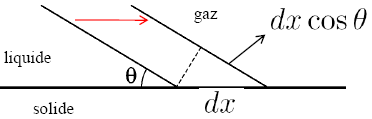
\includegraphics[scale=0.4]{cp/image15.png}
\captionof{figure}{Augmentation $S_{liq}$}
\end{wrapfigure}
La ligne de contact se situe entre les trois phases alors que c'est l'angle de contact $\theta$ qui caractérise les interactions moléculaires entre solide, liquide et gaz.\\

Si on déplace la ligne de contact dans le but d'agrandir la surface du liquide, la tension superficielle $\gamma_{sl}$ augmente alors que $\gamma_{sl}$ diminue.\\
L'énergie $dF$ peut être ainsi écrite\footnote{On peut également obtenir ce résultat par $\sum F = 0$, cf. slide.} : $dF = (\gamma_{sg} - \gamma_{sl})dx + \gamma dx.\cos\theta = 0$\footnote{dF = 0 car F possède un minimum pour $T$ et $V = cste$}. En isolant $\theta$ on trouve la \textbf{loi de Young-Dupré} :
\begin{equation}
\cos\theta = \frac{\gamma_{sg} - \gamma_{sl}}{\gamma}
\end{equation}

\newpage
\subsubsection{Montée capillaire}
\begin{wrapfigure}[9]{r}{2cm}
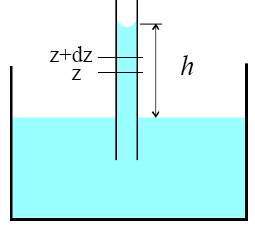
\includegraphics[scale=0.4]{cp/image16.png}
\captionof{figure}{Montée capillaire}
\end{wrapfigure}
L'énergie potentielle ($mgh$) d'une colonne de liquide (rayon $r$) vaut :
\begin{equation}
\int dm(z).g.z = \int_0^h (\rho \pi r^2.dz).g.z = \frac{\rho g \pi r^2 h^2}{2}
\end{equation}

En suivant le même raisonnement que la page ci-dessus on trouve que l'énergie de surface due aux interactions avec la paroi vaut : $2\pi r h(\gamma_{sl}-\gamma_{sg}) + Cste$.\\
$F = U + T.S$ où $U$ peut être vu comme l'énergie de surface et l'énergie potentielle et $T*S$ comme étant constante. Dès lors : 
\begin{equation}
F = 2\pi r h(\gamma_{sl}-\gamma_{sg}) + \frac{\rho g \pi r^2 h^2}{2} + Cste
\end{equation}
En minimisant $F$ par rapport à $H$ : $dF/dh = 2\pi r h(\gamma_{sl}-\gamma_{sg}) + \rho g \pi r^2 h = 0$. En isolant $h$ on retrouve la \textbf{loi (de Jurin) de la montée capillaire :}
\begin{equation}
h = \frac{2(\gamma_{sg}-\gamma_{sl}}{\rho g r} = \frac{2\gamma \cos\theta}{\rho g r}
\end{equation}
L'interprétation physique est simple : la montée est défavorisée par la masse, la gravité et son rayon interne.

\section{Systèmes à plusieurs constituants}
\subsection{Théorèmes d'Euler}
Tentons de généraliser les relations vues au cas de $c > 1$ constituants. Démontrons d'abord deux théorèmes d'Euler qui seront utiles. Soit  une fonction \textbf{extensive} quelconque : $Y(T, p, n_1, \dots, n_c)$. Par def de la variable extensive :
\begin{equation}
Y(T, p, kn_1, \dots, kn_c) = kY(T, p, n_1, \dots, n_c)\ \ \forall k
\end{equation}
On remarque que l'on peut retrouver $Y$ grâce à la relation suivante en effectuant les dérivées de part et d'autre :
\begin{equation}
Y = \sum_{\gamma = 1}^{\gamma = c} \frac{\partial T}{\partial (kn_\gamma)}\frac{\partial (kn_\gamma)}{\partial k}
\end{equation}
Le \textbf{théorème d'Euler pour les fonctions extensives} s'énonce dès lors :
\begin{equation}
Y = \sum _{\gamma = 1}^{\gamma = c} n_\gamma y_\gamma
\end{equation}
où $y_\gamma = \left(\dfrac{\partial Y}{\partial n_\gamma}\right)_{T,p,n'_\gamma}$. Pour une grandeur extensive : $y(T, p, kn_1,\dots, kn_c) = y(T, p,n_1,\dots, n_c)$ on aura le \textbf{théorème d'Euler pour les fonctions intensives} :
\begin{equation}
\sum_{\gamma = 1}^{\gamma = c} n_\gamma\left(\dfrac{\partial y}{\partial n_\gamma}\right)_{T, p, n'_\gamma} = 0
\end{equation}
\subsection{Application du théorème}
Si $Y = G$, on peut généraliser l'énergie libre de Gibbs : $G = \sum n_\gamma \mu_\gamma$ où $\mu_\gamma = \partial G / \partial n_\gamma$. On peut également généraliser $V, H$ et $C_p$ :
\begin{equation}
V = \sum_{\gamma = 1}^{\gamma = c} n_\gamma v_\gamma\ \ \ \ \ \ \ \ \ \ 
H = \sum_{\gamma = 1}^{\gamma = c} n_\gamma h_\gamma\ \ \ \ \ \ \ \ \ \ 
C_p = \sum_{\gamma = 1}^{\gamma = c} n_\gamma C_{p,\gamma}
\end{equation}
Effectuons la différentielle totale de $G(T, p, n_1,\dots, n_c)$ :
\begin{equation}
dG = \left( \frac{\partial G}{\partial T} \right)_{p,n_\gamma} dT + \left( \frac{\partial G}{\partial p} \right)_{T,n_\gamma} dp + \sum_\gamma \left( \frac{\partial G}{\partial n_\gamma} \right)_{T, p, n'_\gamma} dn_\gamma
\end{equation}
On sait que si $dn_\gamma = 0 \rightarrow dG = -sdT + Vdp$. Comme nous volons généraliser, on considère $dn_\gamma \neq 0$. En connaissant la valeur des dérivées de (1.26)\footnote{$G(T,p,n) = U + pV - TS + n.\mu$} on peut généraliser :
\begin{equation}
dG = -S dT + V dp + \sum_\gamma dn_\gamma
\end{equation}
On peut généraliser d'avantage en considérant un système formé de plusieurs phases $G = \sum_\alpha G^\alpha(T, p, n_1^\alpha, \dots, n_c^\alpha)$ où $\mu_\gamma^\alpha$ est le potentiel chimique de $\gamma$ dans la phase $\alpha$. Cela donne :
\begin{equation}
dG = -SdT + Vdp + \sum_\alpha \sum_\gamma \mu_\gamma^\alpha dn_\gamma^\alpha
\end{equation}

\subsection{Conditions d'équilibre physico-chimique}
On sait bien qu'à $P$ et $T = cste$ on obtient un minimum d'énergie libre de Gibbs. S'ils sont bien constant, l'expression ci-dessus devient :
\begin{equation}
(dG)_{T, p} = 0 \ \ \ \ \Rightarrow\ \ \ \ \sum_\gamma \mu_\gamma dn_\gamma = 0
\end{equation}

Ce qui est la \textbf{condition générale d'équilibre physico-chimique}. Cette condition s'applique \textit{aussi bien aux équilibres des réactions chimiques qu'aux équilibres entre phases}.\\

Dans les slides, on donne comme exemple un mélange de deux liquides miscibles en équilibre avec la vapeur. On en arrive à une généralisation de la condition d'équilibre entre phases d'un corps pur : $\mu_A^1 = \mu_A^2$ \textbf{et} $\mu_B^1 = \mu_B^2$.

\section{Propriétés des potentiels chimiques}
Cherchons à établir une relation donnant un lien entre les potentiels chimiques. On a : $dG = -S dT + V dp + \sum_\gamma dn_\gamma$ et $G = \sum_\gamma \mu_\gamma dn_\gamma \Rightarrow dG = \sum_\gamma n_\gamma d\mu_\gamma + \sum_\gamma u_\gamma dn_\gamma$. En égalisant les deux expressions, on retrouve ce lien connu sous le nom de \textbf{relation de Gibbs-Duhem} :
\begin{equation}
SdT - Vdp + \sum_\gamma n_\gamma d\mu_\gamma = 0
\end{equation}
On retrouve les relations précédentes :
\begin{equation}
S = - \left(\frac{\partial G}{\partial T}\right)_{p, n_\gamma}\ \ \ \ \ \  V =  \left(\frac{\partial G}{\partial p}\right)_{T, n_\gamma}\ \ \ \ \ \ \ \mu_\gamma = \left(\frac{\partial G}{\partial n_\gamma}\right)_{T, p, n_\gamma}
\end{equation}
En formant les dérivées croisées (règle de Maxwell) on trouve la généralisation des résultats obtenus pour les corps purs :
\begin{equation}
\left\{\begin{array}{l}
\left( \dfrac{\partial \mu_\gamma}{\partial T} \right) = -s_\gamma\\
\left( \dfrac{\partial \mu_\gamma}{\partial p} \right) = v_\gamma
\end{array}\right.
\end{equation}
\subsection{Variation avec la pression}
\textbf{A compléter !!}

\subsection{Variation avec la température}
\textbf{A compléter !!}\\
Citions néanmoins la relation de Gibbs-Helmholtz (résultat démontré sur le slide, mais je n'étais que physiquement présent à ce moment la) :
\begin{equation}
\left(\frac{\partial \mu_\gamma/T}{T}\right)_{p, n_\gamma} = -\frac{h_\gamma}{T^2}
\end{equation}
Cette relation est plus pratique à utiliser que $\left(\frac{\partial \mu_\gamma}{T}\right)_{p, n_\gamma} = -s_\gamma$, les entropies étant difficilement mesurables.

\subsection{Variation avec la composition}
\subsubsection{Systèmes idéaux}
Il faut avant tout procéder à une classification en définissant le titre molaire, soit $x_\gamma = \dfrac{n_\gamma}{n}$ avec $ n = \sum_\gamma n_\gamma$, le nombre de mole total.
Un \textbf{système idéal} est, par \textit{définition} un système ou tous les potentiels chimiques ont la forme : 
\begin{equation}
\mu_\gamma = \underbrace{\zeta_\gamma(T,p)}_1 + \underbrace{RT\ln(x_\gamma)}_2\ \ \ \ \ \ \text{où :}
\end{equation}
\begin{enumerate}
\item \textit{Partie propre} : ne dépend de la substance et de l'état considéré\footnote{C'est noté l'inverse dans les slides, mais il a pourtant dit ceci..}
\item \textit{Potentiel chimique du mélange} : dépend de la composition
\end{enumerate}
\begin{proof}
\ \\ Nous savons que
\begin{equation}
\left( \dfrac{\partial \mu_\gamma}{\partial p} \right) = v_\gamma = v_\gamma
\end{equation}
Or, nous savons également :
\begin{equation}
v_\gamma = \frac{RT}{p}
\end{equation}
Il en résulte que :
\begin{equation}
\int \frac{d\mu}{dp} = \int \frac{RT}{p} = RT\ln(x_\gamma) + cste
\end{equation}
La constante étant une fonction de $P$ et $T$, il en résulte le résultat attendu :
\begin{equation}
\mu_\gamma = \zeta(T,p) + RT\ln(x_\gamma)
\end{equation}
\end{proof}
Les \textit{mélanges de gaz parfait} sont des systèmes idéaux : $\mu_\gamma = \eta_\gamma (T) + RT\ln(p_\gamma)$.\\
En effet, comme $p_\gamma = x_\gamma p$ on a $\mu_\gamma = \overbrace{\eta_\gamma(T) + RT\ln(p)}^{\zeta_\gamma(T,p)} + RT\ln(x_\gamma)$.\\

Les \textit{solutions suffisamment diluées} vérifient expérimentalement cette loi. Soit $\gamma = 1$ un solvant et $\gamma = 2, \dots, c$ solutés. La solution sera suffisamment diluée si $x_1 \approx 1$ ce qui implique que $x_{\gamma > 1} << 1$.

\subsubsection{Système non-idéaux}
Par définition, on écrit : 
\begin{equation}
\mu_\gamma = \zeta_\gamma(T,p) + RT\ln(a_\gamma)
\end{equation}
où, par définition, le \textit{coefficient d'activité }vaut : $f_\gamma = \dfrac{a_\gamma}{x_\gamma}$ où $a_\gamma$ est l'\textbf{activité}.\\
Pour que $\zeta$ soit toujours défini, on choisira un système formé des même constituants mais placé dans les condition tel qu'il se comporte comme idéal :  $\mu^*_\gamma = \zeta(T,p) + RT\ln(x_\gamma)$ définissant ainsi tous les $\zeta$.

\section{Équilibre chimique}
Prenons une réaction chimique quelconque : 
\begin{equation}
\nu_A R_A + \nu_B R_B + \dots \rightleftharpoons \nu_E P_E + \nu_F P_F + \dots
\end{equation}
Pour $T, p$ fixé, on évolue vers le minimum de $G(T,p,n_1, ..., n_c)$ avec $n_\gamma = n_\gamma^0 + \nu_\gamma\xi$ ou $n_\gamma^0$ est le nombre initial de moles de $\gamma$ qui définit le degré d'avancement $\xi$ de la réaction et ses coefficients stœchiométriques $\nu_\gamma$ :
\begin{itemize}
\item $\nu_\gamma > 0$ pour les produits
\item $\nu_\gamma < 0$ pour les réactifs
\end{itemize}
Dérivons $G$ par rapport à $\xi$ et multiplions et divisons par $\partial n_\gamma$ :
\begin{equation}
\left(\frac{\partial G}{\partial\xi}\right)_{T,p} . \frac{\partial n_\gamma}{\partial n_\gamma} = \sum_\gamma \left(\frac{\partial G}{\partial n_\gamma}\right).\frac{\partial n_\gamma}{\partial\xi} = -A(T,p,\xi)
\end{equation}
En dérivant l'expression de $n_\gamma$\footnote{$\nu_\gamma$ est le rapport du $\Delta$ nombre de moles sur le degré d'avancement} par rapport à $\xi$, que la dérivée de $G$ par rapport à $n_\gamma$ donne $\mu_\gamma$ on trouve l'\textbf{affinité de la réaction chimique considérée :}
\begin{equation}
A = - \sum_\gamma \nu_\gamma \mu_\gamma
\end{equation}
\begin{itemize}
\item $A > 0$ : conversion réactifs $\rightarrow$ produits
\item $A > 0$ : conversion produits $\rightarrow$ réactifs
\item $A = 0$ : équilibre
\end{itemize}
En multipliant cette fois-ci $\dfrac{dG}{d\xi}$ par $\dfrac{d\xi}{d\xi}$ on trouve :
\begin{equation}
-A(\xi)\frac{d\xi}{dt} \leq 0
\end{equation}
Cela implique que la vitesse de réaction $d\xi/dt$ a le même signe que $A$. Pour un système non idéal, on remplace l'expression de $\mu_\gamma$ générale dans l'expression obtenue :
\begin{eqnarray}
A &=& - \sum_\gamma \nu_\gamma\zeta_\gamma(T,p) - RT\sum_\gamma v_\gamma \ln(a_\gamma)\\
 &=& \underbrace{-\sum_\gamma \nu_\gamma\zeta_\gamma(T,p)}_1 -\underbrace{RT\ln\left(\Pi_\gamma(a_\gamma^{\nu_\gamma}\right)}_2
\end{eqnarray}
où 1 est l'affinité propre et 2 l'affinité de mélange. On retrouve la définition du \textbf{quotient réactionnel} exprimé au moyen des activités : 
\begin{equation}
Q = \Pi_\gamma \left(a_\gamma^{\nu_\gamma}\right)
\end{equation}
Par définition de la constane d'équilibre : 
\begin{equation}
K(T,p) = \exp\left[\dfrac{A'(T,P)}{RT}\right] = \exp\left[\dfrac{-\sum_\gamma  \nu_\gamma \zeta_\gamma(T,p) }{RT} \right]
\end{equation} 
En isolant $A$, on peut déduire qu'il y aura équilibre ($A = 0$) si $Q = K$ :
\begin{equation}
A = RT \ln\left[\frac{K(T,p)}{Q} \right]
\end{equation}
Deux cas particuliers (système idéaux et gaz parfaits) sont détaillés dans un slide.

\subsection{Variation de l'affinité avec $T$ et $p$}
\subsubsection{Variation avec $T$}
Sachant que $A = -\sum_\gamma \nu_\gamma \mu_\gamma$ en effectuant la dérivée de $A/T$ par $T$ :
\begin{equation}
\left(\frac{\partial A/T}{\partial T}\right)_{p,n_\gamma} = - \sum_\gamma \nu_\gamma \left(\dfrac{\partial \mu_\gamma / T}{\partial T}\right)
\end{equation}

Par la relation de Gibbs Helmoltz on trouve\footnote{Voir slide pour les \textit{Relation de Kirchhoff}} :
\begin{equation}
\left(\frac{\partial A/T}{\partial T}\right)_{p,n_\gamma} = -\dfrac{r_{Tp}}{T^2}\ \ \ \ \ \ \text{où}\  \ \ \ r_{Tp} = \sum_\gamma \nu_\gamma h_\gamma
\end{equation}

\subsubsection{Variation avec $p$}
Le raisonnement est semblable :
\begin{equation}
\left(\dfrac{\partial A}{\partial p}\right)_{T, n_\gamma} = - \sum_\gamma \left(\dfrac{\partial \mu_\gamma}{\partial p}\right)_{T, n_\gamma} = -\Delta Tp\ \ \ \ \ \text{où}\ \ \Delta Tp = \sum_\gamma \nu_\gamma v_\gamma
\end{equation}
Petite info $\left(\dfrac{\partial r_{Tp}}{\partial p}\right)_{T, n_\gamma} \approx 0$ pour (et \textbf{seulement}) les gaz parfaits.\\

Ces relations importantes permettent de calculer les affinités par intégration en fonction de $T$ et $P$ à partir de leur valeur standard $A^0$.\\

Ces même relations peuvent être obtenues avec $A'$.


\subsection{Tension de vapeur des mélanges}
Rappelons la condition d'équilibre chimique généralisée :
\begin{equation}
\sum_{alpha, \gamma} \mu_\gamma^\alpha dn_\gamma^\alpha = 0
\end{equation}
Comme $dn_\gamma ' + dn_\gamma '' = 0 \rightarrow \sum_\gamma dn_\gamma ' (\mu_\gamma ' - \mu_\gamma '') = 0 \rightarrow \mu_\gamma ' = \mu_\gamma ''\ \forall \gamma$ qui n'est rien d'autre que la traduction du fait qu'à l'équilibre, les potentiels des mêmes phases doivent être identiques.\\

Ceci est de la révision de ce qui a été obtenu en BA1 au cours de \textit{Chimie-Générale}. Les démonstrations sont dans les slides et ne sont pas reprises ici.
\subsubsection{Solution parfaites ($\equiv$ idéales $\forall$ composition)}
Dans l'hypothèse du mélange de gaz parfait, la pression partielle est proportionelle au titre molaire (en phase liquide!) :
\begin{equation}
p_\gamma = k_\gamma x_\gamma
\end{equation}
Dans le cas des corps pur, on retrouve la \textbf{loi de Raoult}(solutions parfaites) : 
\begin{equation}
p_\gamma = p^0_\gamma x_\gamma
\end{equation}
Pour le systèmes binaires : 
\begin{equation}
p = p^0_1\underbrace{(1-x_2)}_{x_1} + p_2^0x_2
\end{equation}
On observe donc une variation linéaires entre les tension de vapeurs des corps purs.

\subsubsection{Solutions suffisamment diluées (donc idéales)}
Pour le solvay ($\gamma = 1$), on trouve la loi de Raoult énoncée ci-dessus. Pour le(s) soluté(s) ($\gamma > 1$) on utilisera la \textbf{loi de Henry} :
\begin{equation}
p_s = k_s(T)x_s
\end{equation}

\subsubsection{Solution binaire parfaite}
Le courbe d'ébullition :
\begin{equation}
p = p^0_2x_2' + p_1^0(1-x_2')
\end{equation}

La courbe de rosée :
\begin{equation}
x_2'' = \frac{p_2^0(p-p_1^0)}{p(p_2^0 - p_1^0)}
\end{equation}
\subsubsection{Règle des segments inverses}
Cette règle est tout à fait générale et s'applique également aux autres diagrammes des phases binaires.
\begin{equation}
\frac{n''}{n'} = \frac{x_2' - x_2}{x_2 - x_2''}
\end{equation}

\subsubsection{Azétropes}
Rien de nouveau par rapport au cours de \textit{Chimie Générale}.

\section{Propriétés colligatives}
Une propriété colligative d'une solution chimique est une propriété qui dépend uniquement du nombre et non de la nature des particules de solutés dans la solution. Leur existence est conséquence de la dilution du soluté par le solvant\footnote{Source : wikipedia}.

\subsection{Loi ébullioscopique}
La loi de Raoult ($p_1 = P_1^0x_1$) nous montre que la tension de vapeur augmente par ajouté d'un soluté\footnote{Si le titre de soluté augmente, $x_1$ diminue entraînement une diminution de $p_1$.}. \\
Cela cause une augmentation de la température d'ébullition (ou de vaporisation. Comment calculer cette élévation par ajoute d'une quantité de soluté ? Considérons l'équilibre entre une solution liquide (') et la phase vapeur ('') du solvant pur :
\begin{equation}
\mu'(T,p,x_1') = \mu ''(T,p)
\end{equation}
Généralisons cette égalité par le potentiel généralisé à gauche, et le potentiel d'un gaz parfait à droite :
\begin{equation}
\mu_1^0(T,p) + RT\ln(a_1)(T,p,x_1') = \eta_1(T) + RT\ln(p)\ \ \ \ \ \ \ (1)
\end{equation}
Si le solvant est pur, on peut négliger l'activité pour avoir : 
\begin{equation}
\mu_1^0(T_0,p) = \eta_1(T_0) + RT_0\ln(p)\ \ \ \ \ \ \ \ \ \ \ \ \ \ \ \ \ \ \ \ \ \  \ \ \ \ \ \\ \ \ \ \ \ \ \ (2)
\end{equation}
Considérons à présent le développement en série tronqué au premier ordre suivant : 
\begin{equation}
\frac{\mu_1^0(T,p)}{T} \approx \frac{\mu_1^0(T_0,p)}{T_0} + (T-T_0)\left[\frac{\partial \mu_1^0 / T}{\partial T}\right]_{T = T_0}
\end{equation}
Le relation de Gibbs-Helmholtz nous donne le dernier terme :
\begin{equation}
\frac{\mu_1^0(T,p)}{T} \approx \frac{\mu_1^0(T_0,p)}{T_0}- \frac{h_1'}{T_0^2} (T-T_0)
\end{equation}
En effectuant $(1)/T - (2)/T_0$ et en utilisant le développement tronqué au premier ordre, on obtient la relation :
\begin{equation}
-\frac{h_1'}{T_0^2}(T-T_0) + R\ln(a_1) = -\frac{h_1''}{T_0^2}(T-T_0)
\end{equation}

En définissant la chaleur latente $\mathcal{L}_v = h_1''- - h_1'$, après avoir mis $(T-T_0)$ en évidence  on trouve : 
\begin{equation}
T - T_0 = - \frac{RT_0^2}{\mathcal{L}_v}\ln(a_1)(T,p,x_1')
\end{equation}
Nous allons ici faire un gros cheat. Voici la démonstration de ce gros cheat :
\begin{proof}
On sait que $x_1' = 1 - \sum_s x_s'$. Soit l'approximation du premier ordre :
$$\ln(1+x) = 0 + x + \mathcal{O}(x^2)$$
Dans notre cas $a_1 \approx x_1$, nous avons donc :
$$\ln(a_1) \approx \ln(x_1) = \ln(1 - \sum_s x_s') \approx -\sum_s x_s$$
\end{proof}
L'expression (1.101) devient dès lors :
\begin{equation}
T-T_0 \approx \frac{RT_0^2}{\mathcal{L}_v}\sum_s x_s = \theta_{eb}\overline{m}_{soluté}
\end{equation}
où l'on à:
\begin{equation}
\left\{\begin{array}{l}
\sum_s x_s = \dfrac{\sum_s n_s}{n} \approx \dfrac{\sum_s n_s}{n_1}\\
\overline{m}_{soluté} = \dfrac{\sum_s n_s}{m_1}\\
\theta_{eb} = \dfrac{RT_0^2M_1}{\mathcal{L}} = \dfrac{RT_0^2}{\mathcal{L}^*}
\end{array}\right.
\end{equation}
où $\mathcal{L}^*$ est exprimée en $J.kg^{-1}$.


\subsection{Loi cryoscopique : abaissement de $T_{fusion}$}
En suivant un raisonnement similaire au précédent (cf. slide pour plus de croustillants détails), on trouve la loi cryoscopique :
\begin{equation}
T-T_0 \approx - \frac{RT_0^2}{\mathcal{L}_f}\sum_s x_s = -\theta_{cr}\overline{m}_{soluté}
\end{equation}

\subsection{Pression osmotique}
\begin{wrapfigure}[11]{l}{5cm}
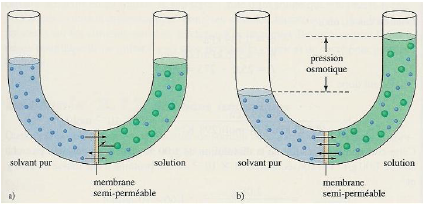
\includegraphics[scale=0.4]{cp/image17.png}
\captionof{figure}{Pression osmotique}
\end{wrapfigure}
Il s'agit d'une autre application des potentiels chimiques, ici pour une solution ('') et un solvant pur (') séparés par une membrane perméable au solvant, mais pas au(x) soluté(s). Cela va causer une élévation du côté de la solution qui peut être transformé en pression : $\pi$.
\begin{equation}
\mu_1^0(T,p) = \mu_1''(T,p+\pi, x_s)
\end{equation}
Si $\pi$ est petit, on peut utiliser le développement de Taylor d'ordre 1\footnote{La dérivée de $\mu$ par rapport à $p$ est $v$}
\begin{equation}
\mu_1^0(T,p) = \mu_1''(T,p+\pi, x_s) \approx \mu_1''(T,p,x_s) + v_1'' \pi
\end{equation}
En mettant le potentiel sous sa forme générale 
\begin{equation}
\mu_1''(T,p,x_s) + v_1'' \pi = \mu_1^0(T,p) + RT\ln(a_1) + v_1''\pi
\end{equation}
En remplaçant dans la première égalité, les $\mu_1^0(T,p)$ s'annulent. En isolant $\pi$ et en utilisant le cheat utilisé un peu plus haut on trouve la \textbf{loi de Van't Hoff} :
\begin{equation}
\pi = -\frac{RT}{v_1''}\ln(a_1) \approx \frac{RT}{v_1^0}\sum_s x_s \approx RT \sum_s C_s
\end{equation}

\section{Équilibres solution - cristaux et miscibilité partielle}
\subsection{Courbe de cristallisation}
Tentons de généraliser le calcul de l'équilibre entre une solution et un solide formé de solvant pur\footnote{Rappel : $T_0 \equiv \mu_1^{0,liq}(T_0,p) = \mu_1^{0,sol}(T_0,p)$} :
\begin{equation}
\mu_1^{0,liq}(T,p) + RT\ln(a_1)(T,p,x_1) = \mu_1^{0,sol}(T,p)
\end{equation}
A la place d'approximer en considérant $T_0$ proche de $T$, intégrons la relation de Gibbs-Helmholtz de $T_0$ à $T$ ce qui donne (ici pour un liquide) :
\begin{equation}
\frac{\mu_1^{0,liq}(T,p)}{T} = \frac{\mu_1^{0,liq}(T_0,p)}{T_0} - \int_{T_0}^T \frac{h_1^{0,liq}}{T^2}dT
\end{equation}
En jouant avec l'expression de $\mathcal{L}_f$ (cf. slide) on retrouve une généralisation de la la loi cryoscopique :
\begin{equation}
R\ln(a_1) = \int_{T_0}^T \frac{\mathcal{L}_f(T)}{T^2}dT
\end{equation}
\end{document}


\part{Applications industrielles}
\setcounter{chapter}{0}
\chapter{Introduction}
\textit{Le génie des procédé à pour but de concevoir et faire fonctionner à l'échelle 
industrielle l'appareillage dans lequel s'effectue les transformations chimique/physique.}

\section{La montée en échelle}


\section{La notion d'opération unitaire}



\section{La démarche du génie des procédés}








\chapter{Distillation}
\section{Introduction}
	\subsection{Equilibre liquide-vapeur : loi de Raoult}
	Etablissons la formulation mathématique des équilibres des potentiels :
	\begin{equation}
	\begin{array}{ll}
	\mu_{A,l}(T,p,x_A) &= \mu_{A,v}(T,p,y_A)\\
	\mu_{B,l}(T,p,x_B) &= \mu_{B,v}(T,p,y_B)
	\end{array}
	\end{equation}
	où $x_{\dots}$ est la fraction molaire liquide et $y_{\dots}$ la fraction molaire 
	liquide. Si l'on associe la vapeur à un gaz parfait, on peut écrire :
	\begin{equation}
	\begin{array}{ll}
	\zeta_{A,l} (T,p) + RT\ln(x_A) &= \xi_A(T) + RT\ln(p_A)\\
	\zeta_{B,l} (T,p) + RT\ln(x_B) &= \xi_B(T) + RT\ln(p_B)	
	\end{array}
	\end{equation}
	Si mon liquide est incompressible, il ne dépend pas de la pression. Dès lors :
	\begin{equation}
	\begin{array}{ll}
	\zeta_{A,l} (T) + RT\ln(x_A) &= \xi_A(T) + RT\ln(p_A)\\
	\zeta_{B,l} (T) + RT\ln(x_B) &= \xi_B(T) + RT\ln(p_B)	
	\end{array}
	\end{equation}
	Si l'on réarrange les termes (je le fais que pour $p_A$, f-l-e-m-m-e) :
	\begin{equation}
	p_A = \exp\left[\dfrac{\zeta_{A,l}(T)-\xi_A(T)}{RT}\right]x_A = f_a(T)x_A :=
	{sat,A}(T)x_A
	\end{equation}
	En en tire la loi de Raoult, ton beau frère :
	\begin{equation}
	\left\{\begin{array}{ll}
	p_A &= p_{sat,A}x_A\\
	p_B &= p_{sat,B}x_B
	\end{array}\right.\ \ \ \ p_A+p_B=p
	\end{equation}
	En pratique, on utilisera Raoult si l'écart des températures est faible. Notons 
	qu'en appliquant cette loi, on se rend compte qu'au sein d'une colonne les zones 
	de compsitions différentes ne peuvent être à la même température car si tel était 
	le cas on n'aurait pas la même pression.\\
	$\rightarrow$\footnote{sp0il} la pression au sein d'une colonne à distiller étant 
	uniforme, la température ne peut l'être (graphe page 12).\\
	
	La loi de Raoult n'est plus valable si on constate qu'elle diverge trop des 
	expérimentations. Deux cas sont alors possibles :
	\begin{enumerate}
	\item Si la pression est inférieure aux prévisions de Raoult
		\begin{itemize}
		\item Dérivation négative : $A$ et $B$ s'attirent $\rightarrow$ évaporation plus
		difficile (azéotrope positif)
		\end{itemize}
	\item Si la pression est supérieure aux prévisions de Raoult
		\begin{itemize}
		\item Dérivation négative : $A$ et $B$ se repoussent $\rightarrow$ évaporation plus
		simple (azéotrope nétatif)
		\end{itemize}
	\end{enumerate}
	
	L'établissement de cette loi permet de définir simplement la pression partielle :
	\begin{equation}
	y_A = \frac{p_A}{p} = \frac{p_{sat,A}(T)x_A}{p_{sat,A}(T)x_A+p_{sat,B}(T)x_B} = \frac{
	\alpha x_A}{\alpha x_A +(1-x_A)}
	\end{equation}
	où $\alpha = \frac{p_{sat,A}(T)}{p{sat,B}(T)}$.
	
	\subsection{But de la distillation}
	Par évaporation succesive d'un mélange liquides dont les composants ont des températures
	d'ébullitions différentes, on est capable d'isoler les différents compsés du mélange.\\
	Ce procédé est utilisé par $\pm 80\%$ des unités de séparations industrielles. Notons 
	tout de même que \textit{séparer} $\neq$ \textit{composition de phase liquide}.
	
	

\section{Procédés de distillation}
	\subsection{Procédé de distillation discontinue}
	\subsection{Procédé de distillation continue}
	
\section{Dimmensionnement d'une installation de distillation discontinue}
	\subsection{Bilan}
	Le nombre de mole du composant liquide étant noté $S(x)$, établissions le bilan
	suivant :
	\begin{equation}
	S(t+\Delta t) = S(t)-\frac{Q'\Delta t}{L}
	\end{equation}
	où le membre de droite signifie \textit{ce qu'il y avait initialement - ce qui s'est 
	évaporé.} En divisant par $\Delta T$ on trouve l'expression différentielle :
	\begin{equation}
	\frac{dS}{dt} = -\frac{Q'}{L}\ \ \rightarrow\ \ S_0-S_f = \frac{Q'}{L}t_f
	\end{equation}
	
	\subsection{Equations constitutives}
	Afin d'établir les équations consitutives de la distillation, il faut à nouveau 
	partir d'un bilan : \textit{Nombre de moles de A dans la cuve = nombres de moles 
	à l'instant suivant + celles évaporée durant ce laps de temps} :
	\begin{equation}
	x(t)S(t) = x(t+\Delta t)S(t+\Delta t) + \left[S(t)-S(t+\Delta t)\right]y(t+\theta
	\Delta t)
	\end{equation}
	où $0\leq\theta\leq 1$. En réorganisant les termes:
	\begin{equation}
	\frac{S(t+\Delta t) -S(t)}{\Delta t}y(t+\theta\Delta t) = \frac{x(t+\Delta t)S(t+
	\Delta t) - x(t)S(t)}{\Delta t}
	\end{equation}
	En passant à la limite $\Delta t \rightarrow 0$ et par définition de la dérivée d'
	un produit :
	\begin{equation}
	\frac{dS}{dt}y = \frac{d}{dt}(x.S) = x\frac{dS}{dt} + S\frac{dx}{dt}
	\end{equation}
	Après une belle mise en évidence : 
	\begin{equation}
	S\frac{dx}{dt} = \frac{dS}{dt}(y-x)
	\end{equation}
	En intégrant, on trouve notre \textbf{première équation constitutive pour la 
	distillation} :
	\begin{equation}
	\int_{x_0}^{x_f} \dfrac{dx}{y-x} = \ln\left(\dfrac{S_f}{S_0}\right)
	\end{equation}
	
		\subsubsection{Paramètre important : composition du distillat $x_D$}
		Important car il s'agit de la \textbf{deuxième équation constitutive :}
		\begin{equation}
		x_D = \frac{S_0x_0-S_fx_f}{S_0-S_f} = \frac{x_0-(S_f/S_0)x_f}{1-(S_0/S_f)}
		\end{equation}
	
	\subsection{Cas ideal/non ideal}
		\subsubsection{Cas ideal : Raoult}
		
		\subsubsection{Cas non idéal : loi empirique}
		
	
	
	
	
	
	
	
	
	
	
	
	
	
	
	
	
	
	
	





\chapter{Filtration et fluidisation}
\section{Introduction}
	\subsection{Traitement des eaux usées}	
	\subsection{Equation constitutive : la percolation}
	
\section{Filtration}
	\subsection{Introduction}
	\subsection{Dimmensionnement des filtres discontinus}
	\subsection{Dimmensionnement des filtres continus}
	
\section{Fluidisation}
	\subsection{Introduction}
	\subsection{Dimmensionnement des lits fluidisés}
	
	
\chapter{Cyclones}
\section{Introduction}
	\subsection{Principe des cyclones}
	\subsection{Vitesse de coupe}
	
\section{Dimmensionnement des cyclones}
		\subsubsection{Temps 1}
		\subsubsection{Temps 2}
	









































\end{document}